\section{An abstract machine for switches}
\label{s:absmachine}

%TODO: Maybe we could minipage the two halves of the figure.
\begin{figure*}[!t]
  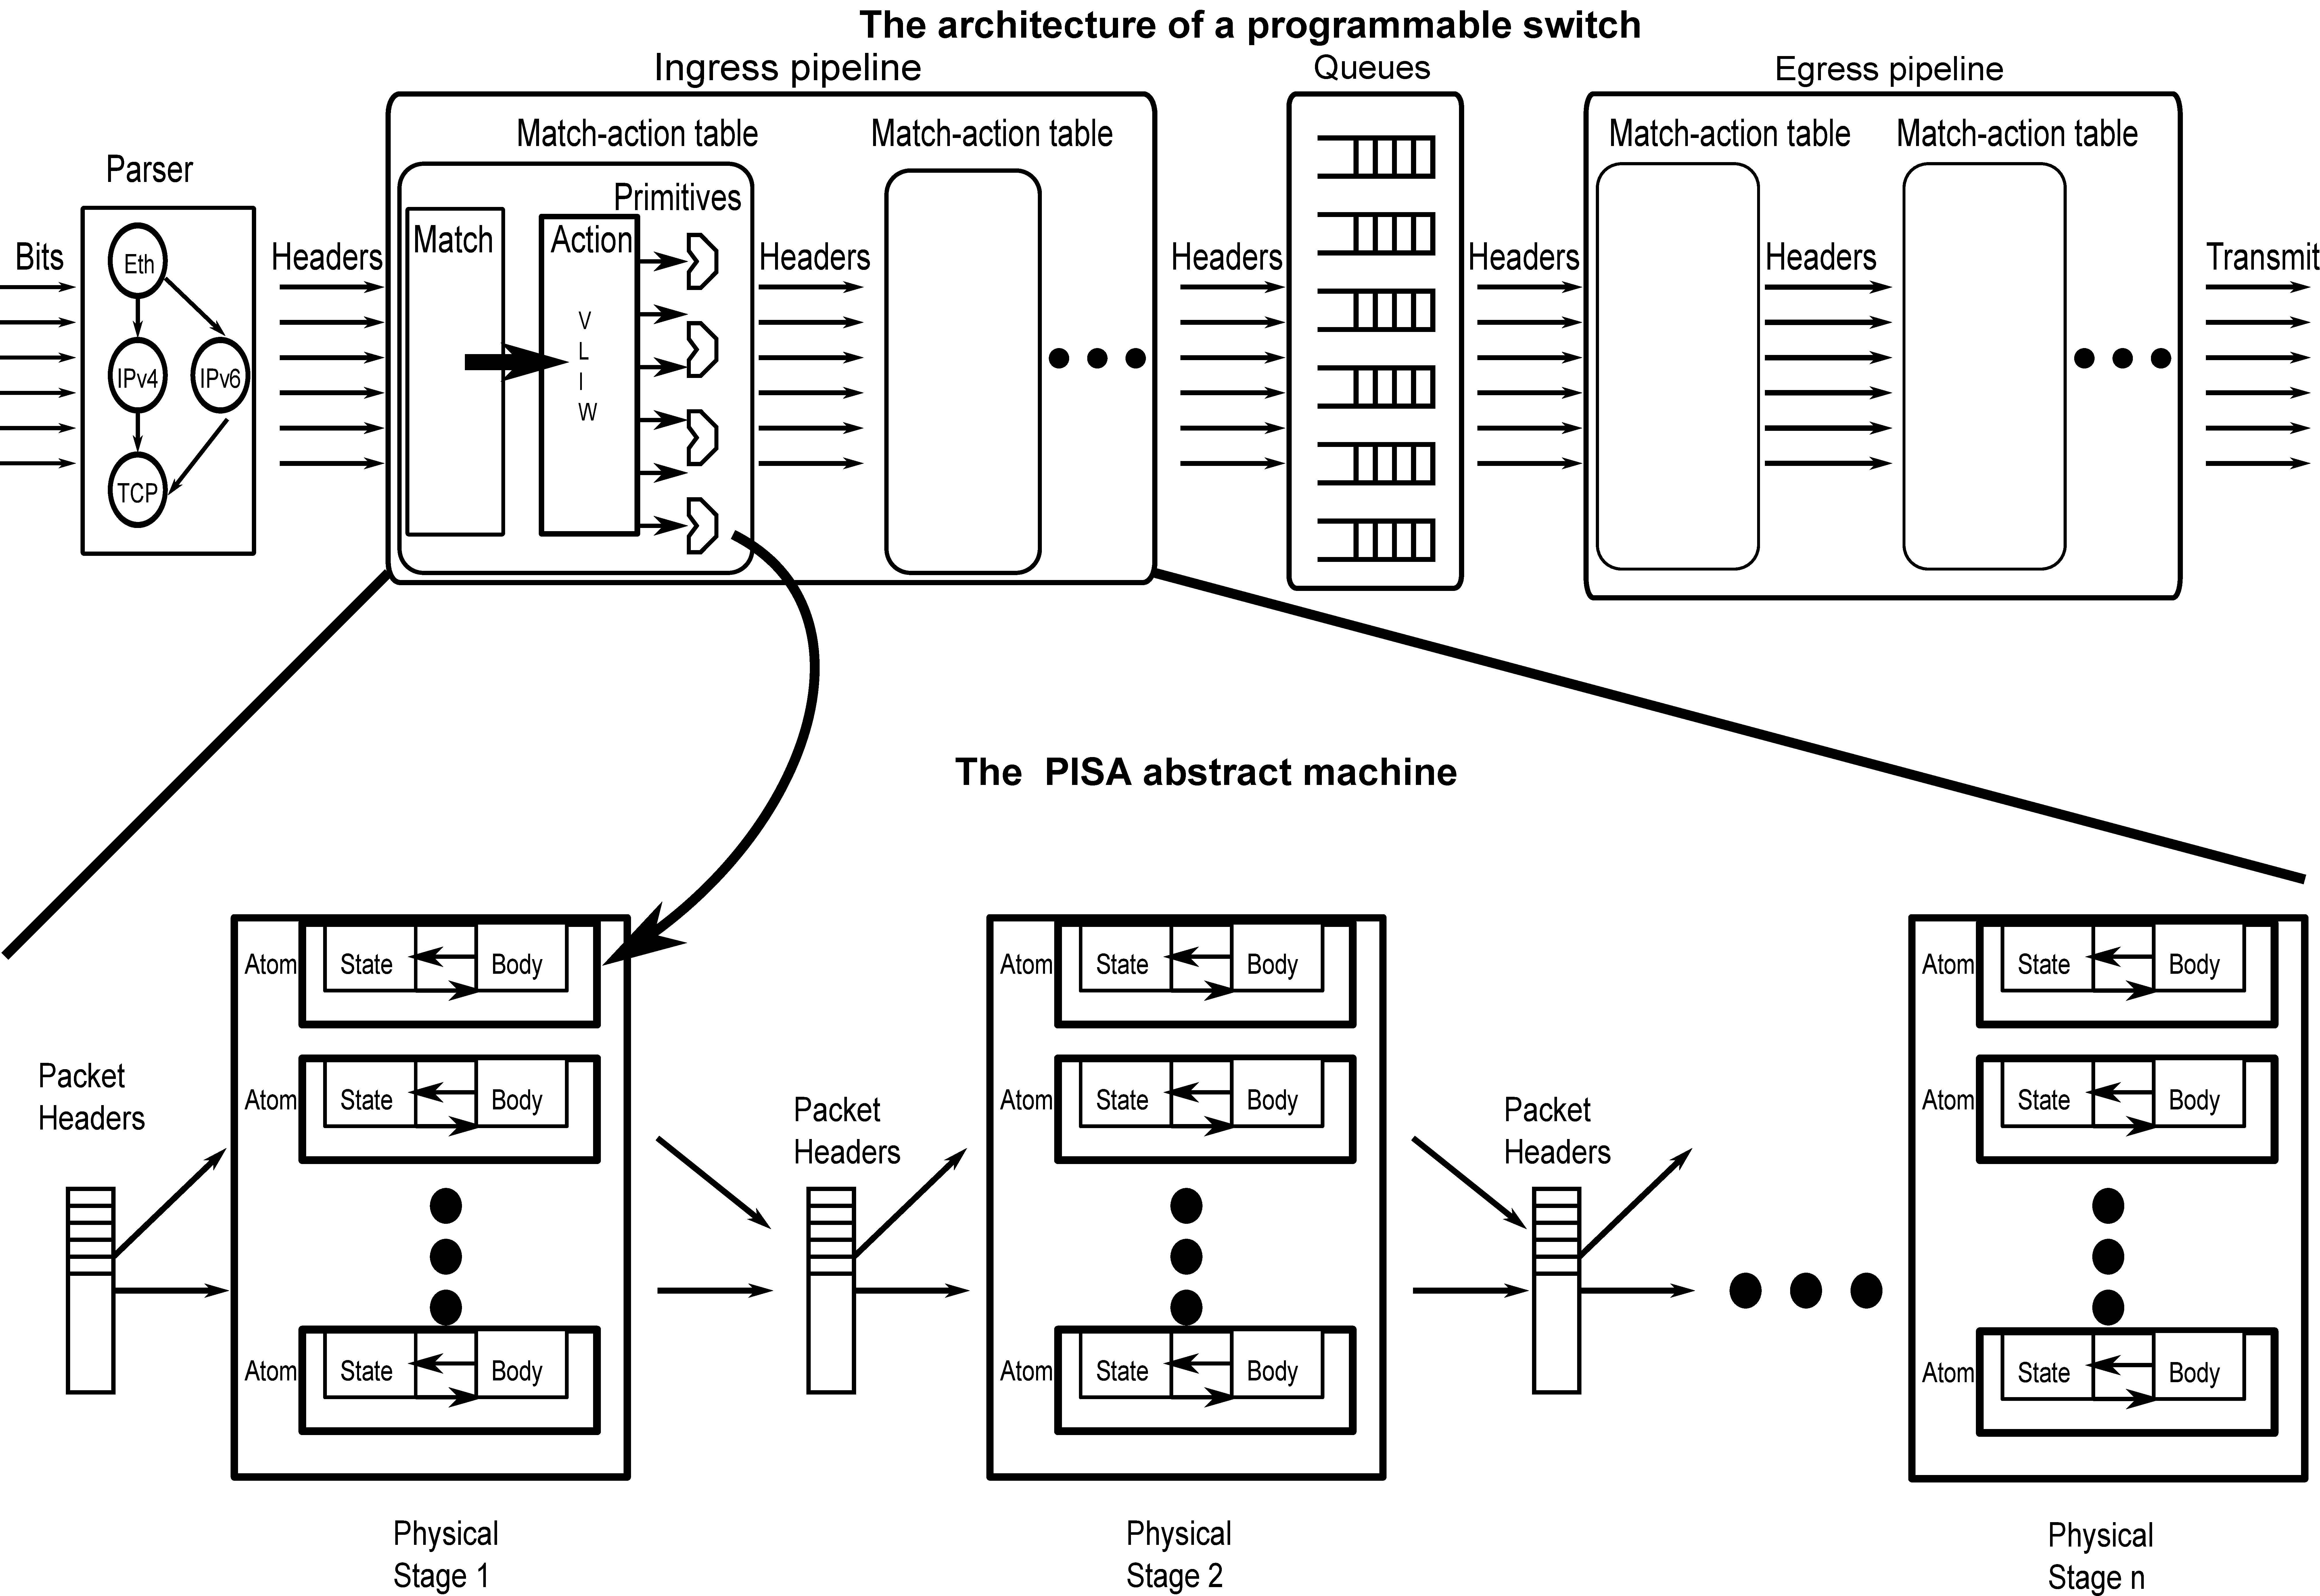
\includegraphics[width=\textwidth]{pisa.pdf}
  \caption{The \absmachine abstract machine and its relationship to
  programmable switch architectures.}
  \label{fig:switch}
\end{figure*}

We first describe \absmachine (Protocol-Independent Switch
Architecture~\cite{nick_p4}), a family of abstract machines that differ in the
computational capabilities they provide. \absmachine machines serve as targets
for \pktlanguage programs. \absmachine's design is inspired by recent line-rate
programmable switch architectures, such as RMT~\cite{rmt}, Intel's
FlexPipe~\cite{flexpipe}, and Cavium's XPliant Packet Architecture~\cite{xpliant}.  These
architectures assume the switch model at the top of Figure~\ref{fig:switch}.

In the top half of Figure~\ref{fig:switch}, packets arriving to the switch are
parsed by a programmable parser that turns packets into header fields. These
header fields are first processed by an ingress pipeline consisting of
match-action tables arranged in stages.  Following the ingress pipeline, the
packet is queued. Once the packet is dequeued by the switch scheduler, it is
processed by a similar egress pipeline before being transmitted from the switch.

\absmachine (the bottom half of Figure~\ref{fig:switch}) models a switch
pipeline such as the ingress or egress pipeline. A pipeline consists of a
number of pipeline stages that execute synchronously on every time step. An
incoming packet is processed by each stage sequentially until it exits the
pipeline. Each stage has one time step of latency, where the time step
is a physical quantity determined by the hardware. The inverse of this time
step is the line rate supported by the pipeline. For instance, the RMT
architecture~\cite{rmt} has a line rate of 960 Million pkts / sec.
% Note to Chang: I hope saying this is ok?
% This is from the SIGCOMM paper and gives away no speeds and feeds.

As an abstract machine, \absmachine only models components pertinent to
data-plane algorithms. In particular, it models the computation within
a match-action table in a stage (i.e., the action half of the match-action
table), but not the match semantics (e.g., direct, ternary, or longest prefix).
\absmachine also does not model packet parsing and assumes that packets
arriving to it are already parsed.

%%\ac{so is pipeline stage a concept in actual
%%hardware switches or is this something invented in \absmachine? The description 
%%in two paragraphs earlier seem to imply former, but last paragraph implies the latter.}
%%Anirudh: Both. We are deriving an abstract model, based on a real switch and we choose
%% to model the pipeline stage explicitly.

\subsection{Atoms: \absmachine's processing units}

%\ac{you mean hardware? otherwise what
%does 'provided natively' mean?}
% changed it to support natively. Hopefully that sounds better.
In \absmachine, each pipeline stage contains a vector of \textit{atoms}. All
atoms in this vector execute in parallel whenever the given stage executes.
Informally, an atom is an atomic unit of packet processing, which the
\absmachine machine supports natively in hardware, and is represented as a body
of sequential code. An atom completes execution of this body of code and
modifies a packet before processing the next packet.  An atom
may also contain internal state that persists across packets and influences the
atom's behavior from one packet to the next.  For instance, a switch counter that
wraps around at 100 can be written as the atom below.\footnote{We use {\tt p.x} to represent
  field {\tt x} within a packet {\tt p} and {\tt x} to represent the state
variable {\tt x} that persists across packets.}
  \begin{lstlisting}[style=customc, numbers=none, frame=none]
  if (counter < 99)
    counter++;
  else
    counter = 0;
  \end{lstlisting}
Similarly, a stateless operation that sets a packet field (such as P4's {\tt
modify\_field} primitive~\cite{p4spec}) can be written as the atom below:
\begin{lstlisting}[style=customc, numbers=none, frame=none]
  p.field = value;
\end{lstlisting}

% Anirudh->Alvin: There is no "instruction set" for the atoms. The atoms are
% the instruction set and you can write whatever you want in them.
% All I care about is that their execution time is bounded. I can't get too
% formal about that, which is why the description is rather informal here.

\absmachine generalizes several aspects of existing programmable switch
architectures. The vector of atoms in each stage generalizes RMT's very-large
instruction-word (VLIW)~\cite{rmt} that executes primitive actions on packet
fields in parallel. Internal state within an atom models persistent switch
state such as meters, counters, and P4's register abstraction~\cite{p4spec} in
a unified manner. We assume all state is initialized by the switch control
plane, which we don't explicitly model in \absmachine.

\subsection{Constraining atoms}
\label{s:atomConstraints}

%Anirudh->Alvin: Hopefully that is cleaerer.
%\ac{I don't see how writing simultaneously at the end of a time step
%prohibits data races.}

Atoms in \absmachine execute on every time step, reading all packet fields at
the beginning and writing all packet fields at the end of a time step. To
prevent data races, \absmachine forbids two atoms in a stage from writing to
the same packet field.  To provide deterministic performance at line rate,
atoms must be suitably constrained.  We impose two such constraints that
distinguish \absmachine from software routers~\cite{click} and network
processors~\cite{ixp4xx} that sacrifice determinism for programmability.

First, \absmachine machines are \textit{shared-nothing}: each atom maintains a
certain number of state variables.  Their values can only be communicated to
atoms in subsequent stages via packet fields. This restriction reflects the
capabilities of line-rate switches: accessing shared memory from multiple
switch stages is technically challenging because it requires multi-ported RAMs
and routing long wires on the chip.

Second, we constrain the complexity of atoms by defining {\it atom templates}
(\S\ref{ss:code_gen}).  Informally, an atom template is a program that always
terminates and specifies how the atom is executed. One example is an ALU with a
restricted set of primitive operations to choose from
(Figure~\ref{fig:alu_in_sketch}). Atom templates allow us to create different
\absmachine machines that support different atoms natively. In practice, we
expect such atom templates be designed by an ASIC engineer and exposed as part
of a \absmachine machine's instruction set. As programmable switches evolve, we
expect the capabilities of atoms to evolve as well. However, atoms cannot be
arbitrarily complex: the line rate is inversely proportional to the maximum
execution latency of all its atoms.
